\newpage
\section{Rationale Zahlen $\mathbb{Q}$}

% ----------------------------------------------------------------------------
\subsection{Definition}

Mit welcher Zahl muss Fünf multipliziert werden, um Zwei zu erhalten?
\[
  5\cdot\square = 2
\]
Diese Frage wird mit Hilfe der Umkehroperation, der Division beantwortet. Als Resultat ergibt sich
\[
  \frac{2}{5} = \square
\]
Dieser Bruch ist aber keine ganze Zahl. Somit kann die Frage innerhalb der ganzen Zahlen nicht beantwortet werden.

Das Problem wird gelöst, indem wiederum neue Zahlen «erfunden» werden.

\textbf{Definition:} Ein Bruch mit ganzen Zahlen in Zähler und Nenner heisst \textbf{rationale Zahl}. Dabei darf der Nenner nicht gleich Null sein. In mathematischer Schreibweise ist $r$ eine rationale Zahl, wenn
  \[
    r := \frac{z}{n} \qquad z,n \in \mathbb{Z},\quad n \ne 0
  \]

Werden alle rationalen Zahlen zusammengefasst, ergibt sich die Menge der rationalen Zahlen.

\textbf{Definition:} Die Menge der rationalen Zahlen ist
  \[
    \mathbb{Q} := \left\{ \frac{z}{n} \qquad z,n \in \mathbb{Z}, \quad n \ne 0\right\}
  \]

\begin{example}
  \textbf{Beispiele:} Einige rationale Zahlen sind
  \[
    \frac{1}{2} \qquad \frac{-4}{-9} \qquad \frac{-5}{10000} \qquad \frac{0}{-2000} \qquad \frac{10}{1}
  \]
\end{example}

\begin{note}
  \textbf{Achtung:} Sogenannte «gemischte Brüche» werden hier nicht definiert. Grundsätzlich sollte die Schreibweise als «gemischter Bruch» vermieden werden, da Sie zu Unklarheiten führen kann. In der Mathematik wird nämlich das Multiplikationszeichen normalerweise weggelassen, nur zwischen zwei Zahlen ist es notwendig. So ist $2a = 2\cdot a$ oder $5\pi = 5\cdot\pi$. Wird nun $2\frac{1}{2}$ geschrieben, so ist unklar, ob dies nun $2+\frac{1}{2}$ oder $2\cdot\frac{1}{2}$ bedeuten soll.

  \textbf{Regel:} Das Additionszeichen darf nicht weggelassen werden, nur das Multiplikationszeichen.
\end{note}

% ----------------------------------------------------------------------------
\subsection{Zahlengerade und Mittelwert}

Auch die rationalen Zahlen lassen sich auf dem Zahlenstrahl darstellen. So befindet sich beispielsweise die Zahl $\frac{1}{2}$ in der Mitte der Zahlen Null und Eins.

\begin{center}
  \begin{tikzpicture}
    \tkzInit[xmin=-2,xmax=2.5,xstep=0.4]
    \tkzDrawX[noticks,label={}]
    \tkzDefPoint(0,0){O}
    \tkzDrawLine({0,-0.1},{0,0.1})
    \tkzLabelPoint({0,-0.1}){$0$}

    \tkzDrawLine({4,-0.1},{4,0.1})
    \tkzLabelPoint({4,-0.1}){$1$}

    \tkzDrawLine({-4,-0.1},{-4,0.1})
    \tkzLabelPoint({-4,-0.1}){$-1$}

    \tkzDrawLine({2,-0.1},{2,0.1})
    \tkzLabelPoint({2,-0.1}){$\frac{1}{2}$}

    \tkzDrawLine({-1.6,-0.1},{-1.6,0.1})
    \tkzLabelPoint({-1.6,-0.1}){$-\frac{2}{5}$}

    \tkzDrawLine({5.33,-0.1},{5.33,0.1})
    \tkzLabelPoint({5.33,-0.1}){$\frac{4}{3}$}
  \end{tikzpicture}
\end{center}

In der Mitte von zwei rationalen Zahlen befindet sich immer deren Mittelwert, der ebenfalls eine rationale Zahl ist. Somit liegen zwischen zwei beliebigen rationalen Zahlen auf dem Zahlenstrahl \textbf{unendlich viele weitere} rationale Zahlen. In der Mathematik wird gesagt, die rationalen Zahlen \textbf{liegen dicht} auf dem Zahlenstrahl.

% ----------------------------------------------------------------------------
\subsection{Abgeschlossenheit}

Die rationalen Zahlen sind bezüglich der folgenden Operationen abgeschlossen:

\begin{itemize}[noitemsep]
  \item Addition
  \item Subtraktion
  \item Multiplikation
  \item Division
\end{itemize}

Das bedeutet, dass die Summe, die Differenz, das Produkt oder der Quotient zweier rationaler Zahlen immer eine rationale Zahl ist.

% ----------------------------------------------------------------------------
\subsection{Äquivalenz}

Brüche können erweitert und gekürzt werden, ohne dass sich deren Wert ändert. Das bedeutet, dass es für jede rationale Zahl unendlich viele verschiedene Darstellungen als Bruch .So ist
\[
  \frac{1}{2} = \frac{2}{4} = \frac{-3}{-6} = \frac{40000}{80000} \cdots
\]

Damit die Darstellung von rationalen Zahlen eindeutig ist, werden folgende Regeln festgelegt:
\begin{itemize}[noitemsep]
  \item Jede rationale Zahl wird durch den \textbf{vollständig gekürzten Bruch} dargestellt.
  \item Ist die rationale Zahl negativ, so wird das \textbf{Minuszeichen vor den Bruch} geschrieben.
  \item Ist der Nenner gleich Eins, wird dieser weggelassen.
\end{itemize}

\begin{example}
  \textbf{Beispiele:}
  \[
    \frac{-4}{-9} = \frac{4}{9}, \qquad \frac{-5}{10} = -\frac{1}{2} \qquad \frac{20}{2} = 10
  \]
\end{example}

% ----------------------------------------------------------------------------
\subsection{Dezimalbrüche}

Jede rationale Zahl kann auch als Dezimalzahl dargestellt werden. Dazu wird das Stellenwertsystem nach rechts erweitert. Rechts von der Stelle Null steht ein Dezimalpunkt, dann folgt die Stelle $-1$, welche einen Stellenwert von $10^{-1}$ oder $\frac{1}{10}$ hat. Wenn wir eine Stelle nach rechts gehen, wird der Stellenwert immer durch Zehn dividiert.

Die Dezimalzahl $42.875$ bedeutet also, dass $4$ Zehner, $2$ Einer, $8$ Zehntel, $7$ Hundertstel und $5$ Tausendstel addiert werden:

\begin{center}[H]
  \renewcommand{\arraystretch}{1.3}
  \newcolumntype{C}{>{\centering\arraybackslash}X}
  \begin{tabularx}{0.9\textwidth}{lCCCCC}
  \toprule
    Stelle & $1$ & $0$ & $-1$ & $-2$ & $-3$ \\
  \midrule
    Stellenwert (Potenz) & $10^{1}$ & $10^{0}$ & $10^{-1}$ & $10^{-2}$ & $10^{-3}$ \\
  \midrule
    Stellenwert & $10$ & $1$ & $\frac{1}{10}$ & $\frac{1}{100}$ & $\frac{1}{1000}$ \\
  \midrule
    Ziffer & $4$ & $2.$ & $8$ & $7$ & $5$ \\
  \midrule
    Wert & $4\cdot 10$ & $2\cdot 1$ & $8\cdot\frac{1}{10}$ & $7\cdot\frac{1}{100}$ & $5\cdot\frac{1}{1000}$ \\
  \bottomrule
  \end{tabularx}
\end{center}

Um einen beliebigen Bruch in eine Dezimalzahl umzuwandeln, wird die schriftliche Division angewendet.
\begin{example}
  \textbf{Beispiele:} Die rationale Zahlen $\frac{1}{8}$, $\frac{2}{3}$ und $\frac{1}{6}$ werden wie folgt als Dezimalbruch dargestellt:
  \[
    \longdivision{1}{8} \qquad\qquad\qquad \longdivision{2}{3} \qquad\qquad\qquad \longdivision{1}{6}
  \]
\end{example}

Manche rationalen Zahlen lassen sich nicht als endliche Dezimalbrüche darstellen, da bei der schriftlichen Division immer ein Rest übrig bleibt. Das heisst, dass sich einige Dezimalstellen unendlich oft wiederholen. Diese werden mit einem Strich oberhalb der Ziffern markiert. Solche Dezimalbrüch heissen \textbf{periodische Dezimalbrüche}.

\begin{example}
  \textbf{Beispiel:} Einige periodische Dezimalbrüche sind:
  \[
    \frac{1}{3} = 0.\overline{3} \qquad
    \frac{1}{6} = 0.1\overline{6} \qquad
    \frac{1}{7} = 0.\overline{142857} \qquad
    \frac{1}{9} = 0.\overline{1} \qquad
    \frac{1}{11} = 0.\overline{09} \qquad
    \frac{1}{13} = 0.\overline{076923}
  \]
\end{example}

Um eine Dezimalzahl in einen Bruch zu verwandeln, rechnen addieren wir einfach die Werte der Dezimalstellen, indem wir die Brüche gleichnamig machen:
\[
  0.875 = \frac{8}{10} + \frac{7}{100} + \frac{5}{1000} = \frac{875}{1000} =\frac{175\cdot 5}{200\cdot 5} = \frac{35\cdot 5}{40\cdot 5} = \frac{7\cdot 5}{8\cdot 5} = \frac{7}{8}
\]
